\documentclass{article}
\usepackage[utf8]{inputenc}
\usepackage[]{graphicx}
\usepackage[margin=1in]{geometry}

\title{Circuits Lab 4}
\author{Theo Thompson and Dan Kearney}
\date{3.3.13}

\begin{document}

\maketitle

\section*{Experiment 1}

\indent Our first experiment compared transistors on the same MAT14 transistor array. For each npn transistor, we tied the collector to the +5V power rail and grounded the emitter. We swept the base voltage from .25V to .65V to characterize the transistor. One way of measuring how well matched transistors are is to measure $\beta$ and $I_{s}$. To do this, we calculated the collector current using KCL: \[I_{e}=I{b}+I_{c}\]
We then calculated $\beta$:\[\beta=\frac{I_{b}}{I_{c}}\]
To calculate $I_{s}$, we used the following relationship: \[I_{c}=I_{s}e^{\frac{V_{be}}{U_{t}}}\]
Where $V_{be}$ is the base-emitter voltage that we sourced with the SMU. The results of our calculation are summarized in the table below.
\begin{center}
    \begin{tabular}{| l | l |} \hline
    $\beta$ & $I_{s}$ \\ \hline \hline
    $875.52$ & $2.01*10^{-13}$ \\ \hline
    $875.64$ & $2.07*10^{-13}$\\ \hline
    $877.97$ & $2.10*10^{-13}$ \\ \hline
    $875.66$ & $2.07*10^{-13}$ \\ \hline
    \end{tabular}
    STD beta: 1.18\\
    STD Is: 3.7749e-15
\end{center}

Beta 


\begin{figure}[h!]
\begin{center}
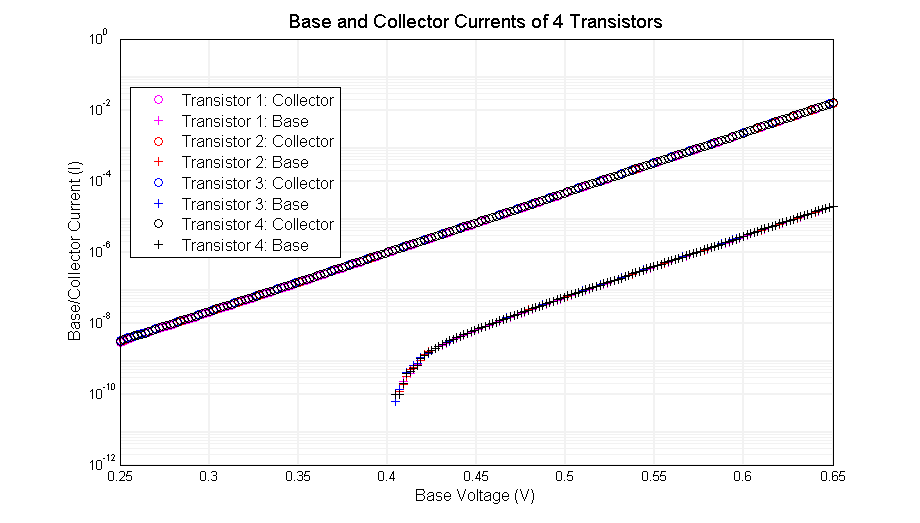
\includegraphics[scale=.6]{exp1a.png}
\caption{}
\label{fig:exp1a}
\end{center}
\end{figure}

\end{document}